
En esta sección se especifican los conjuntos de datos usados en los diferentes modelos.

Los \textbf{modelos no supervisados} utilizarán todo el tablón o mejor expresado, el dataset integrado en su totalidad. Es decir \textit{"baseline\_2009.csv"}. \ref{tablon_integrado} \\

Los \textbf{modelos supervisados} utilizarán el tablón mencionado anteriormente pero dividido en 70\% para train y 30\% para test. A su vez, el conjunto de train puede ser subdividio en train y validation si el modelo lo utiliza.
Los nombres de los conjuntos de entrenamiento y testeo son \textit{"baseline\_2009\_train.csv"} y \textit{"baseline\_2009\_test.csv"} respectivamente.
La generación de dichos conjuntos se realiza en la siguiente sección \ref{dataset_train_test}.\\
Asimismo y según lo obtenido en en análisis de variables importantes \ref{analisis-var_importantes}, ademas de realizar los modelos con todas las variables disponibles, se emplearan modelos con el dataset igualmente distribuido entre train y test pero unicamente utilizando aquellas variables mas importantes.

%-------------------------------------------------%
\subsection{Crear conjuntos de entrenamiento y de prueba}\label{dataset_train_test}
%-------------------------------------------------%

Los conjuntos de train y test se dividen de manera estratificada con la clase y de manera aleatoria con las observaciones. El conjunto train a su vez es subdividido en la etapa de creación de modelos en en train y validation para que en conjunto con técnicas como cross-validation para disminuir o evitar el sobreajuste durante el entrenamiento.\\

La proporción de ambos datasets ha quedado en 56\% de no desertores y 44\% de desertores.



%-------------------------------------------------%
\subsubsection{Otros Datasets}
%-------------------------------------------------%

\paragraph{Reducción de Dimensión: Análisis de Componentes Principales}\label{anuxe1lisis-de-componentes-principales}

Se aplica la técnica de Componentes Principales para reducir la cantidad de variables predictoras pero que a su vez sigan mantengan un gran porcentaje de la variabilidad total.\\
El resultado puede observarse en \ref{fig:pca_varexp_comp}, \ref{tab:loadings_pca_tablon} y \ref{fig:pca_biplot}. Los mismo indican que si bien se puede reducir la cantidad de variables
predictoras y mantener una alta variabilidad de la información
explicada, los diagramas de biplot en este caso no nos servirían de
mucha ayuda ya que en las primeras 2 componentes solo se explica el 41\%
y en las primeras 4 componentes solo el 56\%. Además, los loadings de
dichas componentes no tienen una clara identificación de lo que significan las proyecciónes, por lo que sería complicado explicar el modelo que se quiera desarrollar según estas nuevas variables.

\begin{figure}[!htb]
	\centering
	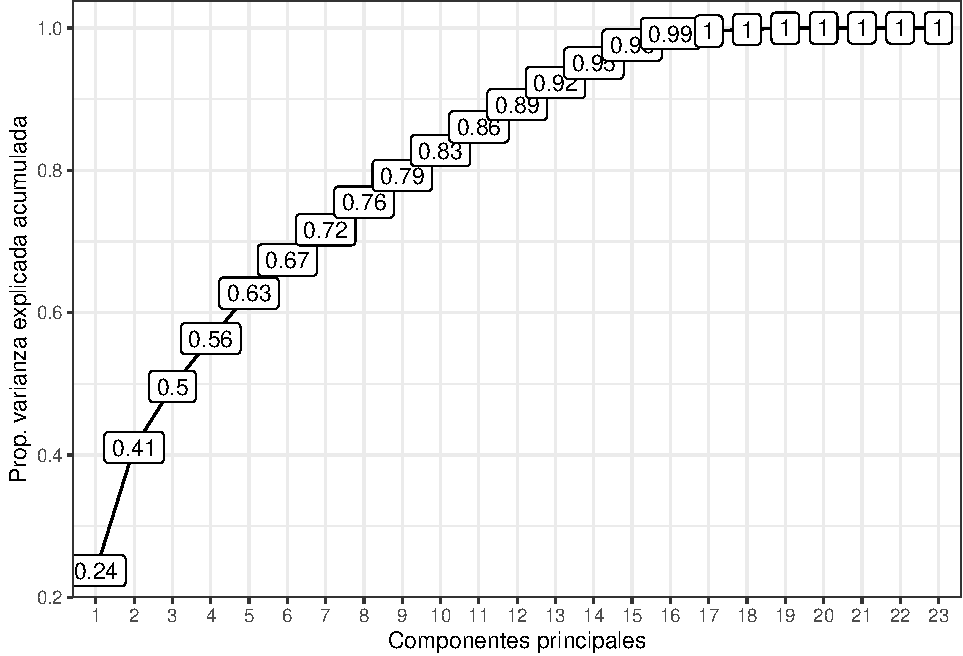
\includegraphics{imagenes/reduccion_dimension/unnamed-chunk-7-1.pdf}
	%\includegraphics[width=0.25\textwidth]{mesh}
	\caption{PCA: Variabilidad explicada VS Componentes}
	\label{fig:pca_varexp_comp}
\end{figure}



\begin{table}[!h]
	
	\caption{\label{tab:loadings_pca_tablon}Loadings de PCA en Tablon}
	\centering
	\begin{tabular}[t]{lrrrr}
		\toprule
		\rowcolor{black}  \multicolumn{1}{c}{\textcolor{white}{\textbf{variable}}} & \multicolumn{1}{c}{\textcolor{white}{\textbf{PC1}}} & \multicolumn{1}{c}{\textcolor{white}{\textbf{PC2}}} & \multicolumn{1}{c}{\textcolor{white}{\textbf{PC3}}} & \multicolumn{1}{c}{\textcolor{white}{\textbf{PC4}}}\\
		\midrule
		\rowcolor{gray!6}  Turno\_Manana & 0.2813063 & -0.1375132 & 0.0171629 & 0.0891187\\
		tipo\_de\_aprobacion\_libre & -0.0516192 & -0.2204644 & -0.1151088 & -0.3721061\\
		\rowcolor{gray!6}  tipo\_de\_aprobacion\_cambio\_curso & 0.0985927 & -0.0960438 & 0.0259816 & -0.0003118\\
		tipo\_de\_aprobacion\_promociono & 0.3581733 & 0.1308245 & -0.0808955 & 0.0804953\\
		\rowcolor{gray!6}  edad\_al\_ingreso & -0.1269356 & 0.0733137 & -0.2349852 & -0.2976394\\
		\addlinespace
		tipo\_de\_aprobacion\_no\_firmo & 0.0156176 & -0.4488391 & -0.1126781 & -0.1126948\\
		\rowcolor{gray!6}  ciclo\_lectivo\_de\_cursada & 0.1818683 & -0.0532719 & -0.1144249 & -0.0532596\\
		tipo\_de\_aprobacion\_firmo & 0.3996032 & 0.0206986 & 0.0690403 & -0.0132481\\
		\rowcolor{gray!6}  cant\_resursada\_regular & 0.0227835 & -0.3127946 & -0.4101361 & 0.3674317\\
		cant\_recursada\_regular\_No\_Recurso & 0.3869691 & 0.1219610 & 0.0468956 & 0.0352279\\
		\addlinespace
		\rowcolor{gray!6}  cant\_recursada\_regular\_Recurso1vez & 0.1188652 & -0.2681558 & 0.0654967 & -0.1891977\\
		cant\_recursada\_regular\_Recurso2vez & 0.0451665 & -0.2939066 & -0.0071695 & -0.1971879\\
		\rowcolor{gray!6}  cant\_recursada\_regular\_Recurso3vez & 0.0120116 & -0.2503402 & -0.0867234 & -0.1612458\\
		cant\_recursada\_regular\_Recurso4vez & 0.0044083 & -0.1971933 & -0.0845225 & -0.1281708\\
		\rowcolor{gray!6}  cant\_recursada\_regular\_Recurso5vez & 0.0006389 & -0.1464459 & -0.1411299 & 0.0048529\\
		\addlinespace
		cant\_recursada\_regular\_RecursoNveces & -0.0021967 & -0.1955233 & -0.4257671 & 0.4879239\\
		\rowcolor{gray!6}  Turno\_Tarde & 0.1153361 & -0.1754377 & 0.0127343 & 0.0859205\\
		Turno\_Noche & 0.2032766 & -0.1098708 & -0.0798642 & -0.3755512\\
		\rowcolor{gray!6}  Aprobado & 0.3918783 & 0.1006967 & -0.0242947 & -0.0374767\\
		Promociono & 0.3589365 & 0.1289055 & -0.0812155 & 0.0798013\\
		\addlinespace
		\rowcolor{gray!6}  noAprobado & 0.2504186 & -0.1806504 & 0.2037648 & -0.0519875\\
		Nota & -0.0001346 & 0.3003970 & -0.4732939 & -0.2012817\\
		\rowcolor{gray!6}  Nota\_max\_prom & 0.0688392 & 0.2670847 & -0.4728596 & -0.2279385\\
		\bottomrule
	\end{tabular}
\end{table}

\begin{figure}[!htb]
	\centering
	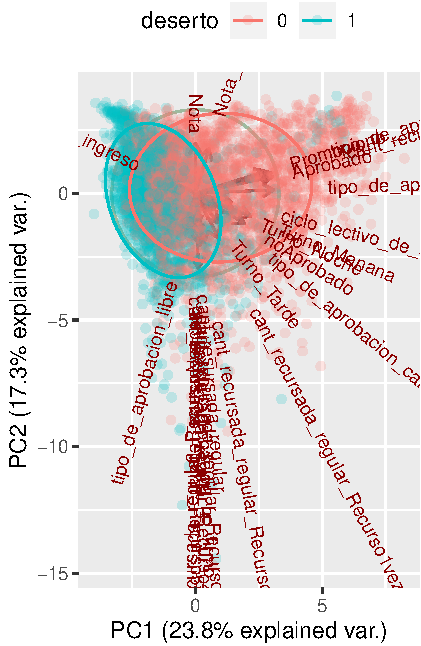
\includegraphics{imagenes/reduccion_dimension/unnamed-chunk-9-1.pdf}
	%\includegraphics[width=0.25\textwidth]{mesh}
	\caption{PCA: biplot PC1 y PC2}
	\label{fig:pca_biplot}
\end{figure}

\paragraph{Reducción de Dimensión: Reducción por t-SNE}\label{reducciuxf3n-por-t-sne}

Al igual que PCA, existen otro algoritmos que pueden realizar reducción
de dimensionalidad. Unos de esos casos es el método no lineal
t-distributed stochastic neighbor embedding (t-SNE), que en ciertos
casos es ventajoso respecto a PCA ya que éste último solo aplica reducción utilizando solamente
combinaciones lineales de las variables originales.\\

Por lo tanto se aplica dicho método de reducción al tablón original y al mismo tiempo se identifican las observaciones según el target real (variable no incluida al hacer la reducción). Cuyos resultados \ref{fig:tsne} indican que si bien no se arman grupos bien definidos,
al identificar cada observación con un color en el gráfico según el
target puede observarse que están mas separadas y hay menos solapamiento entre ellas que con el método PCA. Este resultado puede insinuar que es posible clasificar un gran porcentaje de los casos correctamente a costa quizás de no poder describir o explicar fácilmente como se ha llegado a los resultados.


\begin{figure}[!htb]
	\centering
	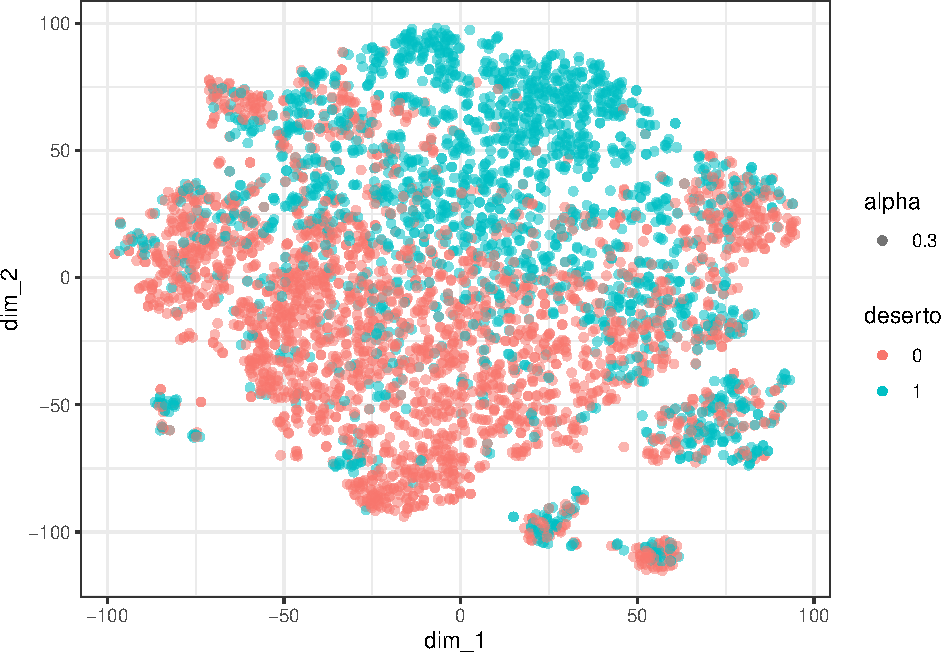
\includegraphics{imagenes/reduccion_dimension/unnamed-chunk-11-1.pdf}
	%\includegraphics[width=0.25\textwidth]{mesh}
	\caption{t-SNE}
	\label{fig:tsne}
\end{figure}

\clearpage




